\begin{figure}[h]
    \centering
    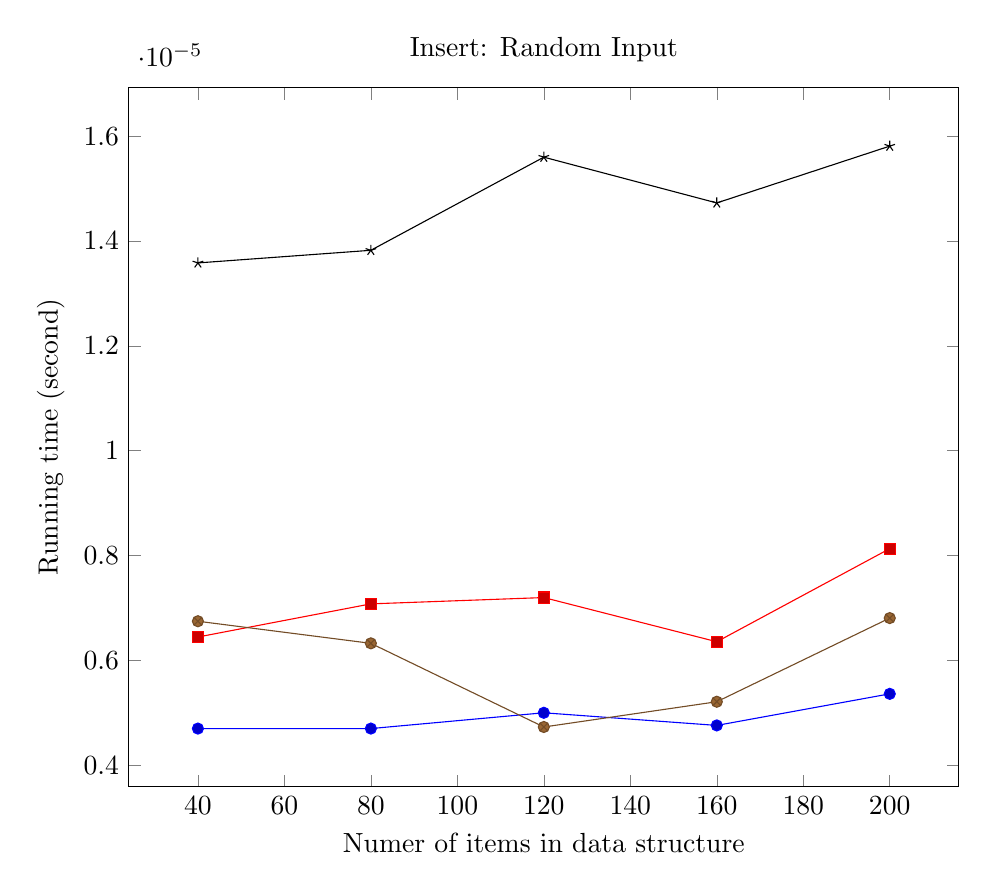
\begin{tikzpicture}
        \begin{axis}[
            xlabel={Numer of items in data structure},
            ylabel={Running time (second)},
            title={Insert: Random Input},
            width=\textwidth
        ]
		\addplot coordinates {
			(40, 4.698335253328079e-06)
			(80, 4.698335253328079e-06)
			(120, 4.999510590075751e-06)
			(160, 4.758570320675948e-06)
			(200, 5.360920994179619e-06)
		};
		\addplot coordinates {
			(40, 6.445152206485671e-06)
			(80, 7.077620413661889e-06)
			(120, 7.198090548363179e-06)
			(160, 6.35479960546248e-06)
			(200, 8.131734092295395e-06)
		};
		\addplot coordinates {
			(40, 6.7463275432361195e-06)
			(80, 6.324682071784382e-06)
			(120, 4.728452787000626e-06)
			(160, 5.210333325805783e-06)
			(200, 6.806562610586764e-06)
		};
		\addplot coordinates {
			(40, 1.3583007687498206e-05)
			(80, 1.382394795690356e-05)
			(120, 1.5600882443736474e-05)
			(160, 1.4727473967154903e-05)
			(200, 1.5811705179460955e-05)
		};
        \legend{}
        \end{axis}
    \end{tikzpicture}
    \caption{Average of 0 operations, benchmarked every 0, starting at 0.}
\end{figure}